%%
%% Modified by Ricardo Garcia-Rosas to satisfy the rules established by the University of Melbourne's Research Higher Degrees Committee as of 4th of June 2019.
%% Guidelines can be found at: https://gradresearch.unimelb.edu.au/__data/assets/pdf_file/0004/2027839/Preparation-of-GR-theses-rules.pdf
%%
%%
%% ----------------------------------------------------------------
%% Thesis.tex -- MAIN FILE (the one that you compile with LaTeX)
%% ---------------------------------------------------------------- 

% Set up the document
\documentclass[a4paper, 11pt, twoside]{Thesis}  % Use the "Thesis" style, based on the ECS Thesis style by Steve Gunn
%
% Put your figures in this directory
\graphicspath{Figures/}  % Location of the graphics files (set up for graphics to be in PDF format)
%

% hide anything lower than section in the TOC
\setcounter{tocdepth}{2}

% Include any extra LaTeX packages required
\usepackage[english]{babel}
% with babel and biblatex, csquuotes is a requirements for quoted text to work as expected
\usepackage{csquotes}

%better fonts
\usepackage{lmodern}

\usepackage[usenames,dvipsnames]{xcolor}

%reference managing
\usepackage[sorting=none, citestyle=numeric, backend=biber]{biblatex}
\addbibresource{MyBibLatex.bib}

% we allow the urls in the bibliography to be broken after normal characters as well, not just '-', '\' and '.'
\setcounter{biburllcpenalty}{7000}
\setcounter{biburlucpenalty}{8000}

\usepackage{verbatim}  % Needed for the "comment" environment to make LaTeX comments


%setup the links the right way
\hypersetup{urlcolor=blue, colorlinks=true}  % Colours hyperlinks in blue, but this can be distracting if there are many links.

%allow short citations in the beginning of chapters
\usepackage{epigraph}
% and set it up
\renewcommand{\epigraphsize}{\small\itshape}
\setlength\epigraphwidth{9.5cm}


%this redefines how chapters look and also allows quotes
\usepackage[avantgarde]{quotchap}
%make the title left justified
\makeatletter
\patchcmd{\@makechapterhead}
 {\raggedleft\advance}
 {\raggedright\advance}
 {}{}
\makeatother
%reduce the spacing after a chapter
\renewcommand{\chapterheadendvskip}{\vspace*{0.7\baselineskip}}




% allow marks and todos !!! REMOVE FOR FINAL VERSION !!!
\setlength{\marginparwidth}{2cm}

\usepackage[colorinlistoftodos, prependcaption,textsize=small]{todonotes}


%allows us to use figures nicer
\usepackage{float}

%allows a nice way to "flush" floats
\usepackage{afterpage}

%% ----------------------------------------------------------------

\begin{document}
\frontmatter      % Begin Roman style (i, ii, iii, iv...) page numbering

%
\UNIVERSITY{{THE UNIVERSITY OF MELBOURNE }}    
%
%%%%%%%%%%%%%%%%%%%%%%%%%%%%%%%%%%%%%%%%%%%%%%%%%%%%%%%%%%%%%%%%%%%%%%%%%
% Update your department and school here:
\department{{Sir Peter MacCallum department of Oncology}}
\school{{Melbourne School of Awesome}}
%%%%%%%%%%%%%%%%%%%%%%%%%%%%%%%%%%%%%%%%%%%%%%%%%%%%%%%%%%%%%%%%%%%%%%%%%

%
%%%%%%%%%%%%%%%%%%%%%%%%%%%%%%%%%%%%%%%%%%%%%%%%%%%%%%%%%%%%%%%%%%%%%%%%%
% Set up the Title Page
% Change your thesis title and your information here
\title  {Circulating tumour DNA for precision medicine in Non-small cell lung cancer}
\authors  {\texorpdfstring
            {\href{https://github.com/sebastianhollizeck}{Sebastian Hollizeck\\ \small ORCID: 0000-0002-9504-3497}}
            {Sebastian Hollizeck}
            }
\addresses  {\groupname\\\deptname\\\univname}  % Do not change this here, instead these must be set in the "Thesis.cls" file, please look through it instead
\date       {\today}
\subject    {}
\keywords   {cancer evolution, cancer heterogeneity, ctDNA, variant calling}
%%%%%%%%%%%%%%%%%%%%%%%%%%%%%%%%%%%%%%%%%%%%%%%%%%%%%%%%%%%%%%%%%%%%%%%%%

\maketitle
%% ----------------------------------------------------------------

\setstretch{1.3}  % It is better to have smaller font and larger line spacing than the other way round

% Define the page headers using the FancyHdr package and set up for one-sided printing
\fancyhead{}  % Clears all page headers and footers
\rhead{\thepage}  % Sets the right side header to show the page number
\lhead{}  % Clears the left side page header

\pagestyle{fancy}  % Finally, use the "fancy" page style to implement the FancyHdr headers

%% ----------------------------------------------------------------
% The Abstract Page
\input{Preamble/Abstract.tex}
\clearpage  % Abstract ended, start a new page

%% ----------------------------------------------------------------
% Declaration Page required for the Thesis, your institution may give you a different text to place here
\input{Preamble/Declaration.tex}
\clearpage  % Declaration ended, now start a new page

%% ----------------------------------------------------------------
% Preface Page required for the Thesis, your institution may give you a different text to place here
\input{Preamble/Preface.tex}
\clearpage  % Preface ended, now start a new page

%% ----------------------------------------------------------------
% The Acknowledgements page, for thanking everyone
\setstretch{1.3}  % Reset the line-spacing to 1.3 for body text (if it has changed)
\input{Preamble/Acknowledgements.tex}
\clearpage  % End of the Acknowledgements
%% ----------------------------------------------------------------

\pagestyle{fancy}  %The page style headers have been "empty" all this time, now use the "fancy" headers as defined before to bring them back


%% ----------------------------------------------------------------
\lhead{\emph{Contents}}  % Set the left side page header to "Contents"
\tableofcontents  % Write out the Table of Contents

%% ----------------------------------------------------------------
\lhead{\emph{List of Figures}}  % Set the left side page header to "List if Figures"
\listoffigures  % Write out the List of Figures

%% ----------------------------------------------------------------
\lhead{\emph{List of Tables}}  % Set the left side page header to "List of Tables"
\listoftables  % Write out the List of Tables

%% ----------------------------------------------------------------
\setstretch{1.5}  % Set the line spacing to 1.5, this makes the following tables easier to read
\clearpage  % Start a new page
\lhead{\emph{Abbreviations}}  % Set the left side page header to "Abbreviations"
\listofsymbols{ll}  % Include a list of Abbreviations (a table of two columns)
{
% \textbf{Acronym} & \textbf{W}hat (it) \textbf{S}tands \textbf{F}or \\
\textbf{DNA} & \textbf{D}eoxyribo\textbf{N}ucleic \textbf{A}cid \\
\textbf{RNA} & \textbf{R}ibo\textbf{N}ucleic \textbf{A}cid \\
\textbf{cfDNA} & \textbf{c}ell \textbf{f}ree \textbf{DNA} \\
\textbf{ctDNA} & \textbf{c}irculating \textbf{t}umour \textbf{DNA}\\
\textbf{bp} & \textbf{b}ase \textbf{p}air\\
\textbf{ChIP} & \textbf{Ch}romatin \textbf{I}mmuno\textbf{P}recipitation\\
\textbf{WGS} & \textbf{W}hole \textbf{G}enome \textbf{S}equencing\\
\textbf{WES} & \textbf{W}hole \textbf{E}xome \textbf{S}equencing\\
\textbf{SCLC} & \textbf{S}mall \textbf{C}ell \textbf{L}ung \textbf{C}ancer\\
\textbf{NSCLC} & \textbf{N}on-\textbf{S}mall \textbf{C}ell \textbf{L}ung \textbf{C}ancer\\
\textbf{RAID} & \textbf{R}edundant \textbf{A}rray of \textbf{I}ndependent \textbf{D}isks \\
\textbf{SNP} & \textbf{S}ingle \textbf{N}ucleotide \textbf{P}olymorphism\\
\textbf{InDel} & \textbf{In}sertion or \textbf{Del}etion \\
\textbf{SV} & \textbf{S}tructural \textbf{V}ariant \\
\textbf{PON} & \textbf{P}anel \textbf{O}f \textbf{N}ormals \\
\textbf{GATK} & \textbf{G}enome \textbf{A}nalysis \textbf{T}ool\textbf{K}it \\
\textbf{NJ} & \textbf{N}eighbour \textbf{J}oining \\
\textbf{UPGMA} & \textbf{U}nweighted \textbf{P}air \textbf{G}roup \textbf{M}ethod with \textbf{A}rithmetic mean \\
\textbf{WPGMA} & \textbf{W}eighted \textbf{P}air \textbf{G}roup \textbf{M}ethod with \textbf{A}rithmetic mean \\
\textbf{F81} & \textbf{F}elsenstein 19\textbf{81} model \\
\textbf{HKY85} & \textbf{H}asegawa, \textbf{K}ishino and \textbf{Y}ano 19\textbf{85} model\\



}

%% ----------------------------------------------------------------
\clearpage  % Start a new page
\lhead{\emph{Constants}}  % Set the left side page header to "Physical Constants"
\listofconstants{lrcl}  % Include a list of Physical Constants (a four column table)
{
% Constant Name & Symbol & = & Constant Value (with units) \\
Speed of Light & $c$ & $=$ & $2.997\ 924\ 58\times10^{8}\ \mbox{ms}^{-\mbox{s}}$ (exact)\\

}

%% ----------------------------------------------------------------
\clearpage  %Start a new page
\lhead{\emph{Symbols}}  % Set the left side page header to "Symbols"
\listofnomenclature{lll}  % Include a list of Symbols (a three column table)
{
% symbol & name & unit \\
$a$ & distance & m \\
$P$ & power & W (Js$^{-1}$) \\
& & \\ % Gap to separate the Roman symbols from the Greek
$\omega$ & angular frequency & rads$^{-1}$ \\
}
%% ----------------------------------------------------------------
% End of the pre-able, contents and lists of things


%% ----------------------------------------------------------------
\mainmatter	  % Begin normal, numeric (1,2,3...) page numbering
\pagestyle{fancy}  % Return the page headers back to the "fancy" style

%setup so that the header shows the chapter and the footer shows the page number
\fancyhead[LE,RO]{\rightmark}
\fancyhead[RE,LO]{}
\fancyfoot[LE,RO]{\thepage}
\fancyfoot[RE,LO]{}

%make pretty lines
%\renewcommand{\footrulewidth}{1pt}
\renewcommand{\headrulewidth}{1pt}

%change the distance of the number to the top of the page
\renewcommand{\chapterheadstartvskip}{\vspace*{-4\baselineskip}}

% Include the chapters of the thesis, as separate files
% Just uncomment the lines as you write the chapters

% main introduction

\begin{savequote}[85mm]
``Begin at the beginning,`` the King said, very gravely, ``and go on till you come to the end: then stop.``
\qauthor{--- Lewis Carroll, \textit{Alice in Wonderland}}
\end{savequote}

\chapter{Introduction}
\label{ch:intro}

%\epigraph{``Begin at the beginning,`` the King said, very gravely, ``and go on till you come to the end: then stop.``}{ --- \textup{Lewis Carroll}, Alice in Wonderland}


This first introduction chapter contains all the necessary background information as well as an overview for the work discussed in this thesis. It summarised basic biological properties of DNA and cell biology as well as the respective technologies to read, analyse and measure these biological concepts and then how to evaluate the output of these methods.
\hyperref[intro-sec:DNA]{Section~\ref*{intro-sec:DNA}} delineates the role DNA plays for the cell and then \hyperref[intro-sec:ctDNA]{section~\ref{intro-sec:ctDNA}} shows how these standards are changed in the tumour and cell free context. \hyperref[intro-sec:sequencing]{Section~\ref{intro-sec:sequencing}} introduces the current technologies used to measure and detect DNA and its variations. With \hyperref[intro-sec:analysis]{section~\ref*{intro-sec:analysis}} covering the computational analysis methods to read out changes in the DNA. Then \hyperref[intro-sec:lungcancer]{section~\ref{intro-sec:lungcancer}} relates how these changes lead to cancer and what we can learn from them. 
The introduction concludes with \hyperref[intro-sec:overview]{section~\ref*{intro-sec:overview}} as an overview over the thesis aims and my work in addressing them in the following chapters.


%%% this just contains all the links and possible formating of the introduction as a whole

% background of DNA
\section[DNA]{DNA as a information storage unit}
\label{intro-sec:DNA}

\begin{figure}[!ht]
\centering
\includegraphics[width=0.9\linewidth]{Figures/DNAStructure}
\caption[Overview DNA structure]{Overview of DNA structure and the nucleobases, which form DNA strands. Nucleotides are split into Purines and Pyrimidines by the structure of the nitrogen ring; complementary pairing of bases is shown as shapes of the bases as well as with 2D structures; Hyrdogen (H) bonds are shown as dotted lines; Phosphates are shown as P; 3' and 5' ends are defined by the internal number of the carbon atom of the sugar which is exposed; Adapted from ``DNA structure`` by \href{https://biorender.com}{\nolinkurl{BioRender.com}} (2021) Retrieved from \href{https://app.biorender.com/biorender-templates}{\nolinkurl{https://app.biorender.com/biorender-templates}}}\label{fig:DNAstructure}
\end{figure}


It is a widely accepted fact, that Deoxyribonucleic acid (DNA) serves as the long term information storage molecule of our cells. This information is protected and allows correction of simple errors through its double helix structure \cite{Watson1953,Liang1998}. The nucleotides, which consist of a deoxyribose sugar (hence the name), a phosphate group and the nitrogenous base, are joined together by phosphate groups. Even though there are six common naturally occurring nitrogenous bases: Adenine (A), Thymine (T), Guanine (G), Cytosine (C), Uracil (U) and nicotinamide, only the first four are used to encode the genetic information into DNA. Each of the strands mirrors the other, so that an adenine will be paired up with a thymine forming two hydrogen bonds. Similarly cytosine will pair with guanine forming an even stronger bond with three hydrogen bonds. While other pairings which do not follow those rules are chemically possible, they are mostly observed in ribonucleic acid (RNA) \cite{Sinden1994}. These very strict bonding rules enable the DNA to be similar to a hard drive with backup on a computer. And as only one strand contains all the information, the DNA polymerase enzyme does only need access to one strand, which allows parallel replication during cell division, but also error corrections, by proof reading the newly synthesised strand with the template. In order to be able to distinguish the two strands, they were assigned the names 3' and 5' depending on the numbering of the carbon atom in the sugar, which is exposed (\autoref{fig:DNAstructure}).

The entirety of the DNA encoding the organism is commonly called ``the genome`` with all genes, which consist of introns and exons are called exome. Unicellular organisms usually only have a very small amount of introns, which to current knowledge only provide limited information and are only responsible for structure. In vertebrates  introns as well as intergeneic DNA (the DNA between genes) contribute most of the DNA in the genome. For example in humans, only $1\%$ of the genetic material is considered to be exonic, whereas introns contribute $\approx 24\%$ and the rest is intergeneic ($\approx 75\%$)\cite{Venter2001}.

\begin{figure}[!ht]
\centering
\includegraphics[width=0.9\linewidth]{Figures/ChromosomeStructure}
\caption[Overview Chromosome structure]{Structural overview of the metaphase condensed chromosome: DNA is first wrapped around Histones to form nucleosome, which then associate with each other to form the chromatin fiber, which in the metaphase of the cell cycle is condensed even more into the X-shaped chromosome}\label{fig:chromsomestructure}
\end{figure}

The DNA in eukaryotes however is not free floating around in the nucleus of a cell, but rather in most eukrayotic organisms, it is highly condensed and structured, first wrapped around nucleosomes like thread on a spool, then organised around histones, into either open (accessible) or closed chromatin, which then can be even further condensed into chromosomes, which have a X-like shape, with two shorter and two longer arms (\autoref{fig:chromsomestructure}). This allows some of the DNA to be accessible where the use of other areas can be restricted\cite{Hammond2017}. Through this restriction, the availability of certain genes, which are the sections of the DNA, which encode for short term storage molecules like RNA. This restriction plays an important role in cell fate and cell viability. Ultimately all information stored to create a new highly complex organism is stored in just the DNA of one cell. Whichever parts are used and how they are used decides the function and the identity of the cell\cite{Bonev2016}. 



\subsection[Ploidy]{Ploidy - its good to have a backup, if you do it right}
\label{intro-sec:ploidy}
Similar to the already discussed RAID-like setup of the DNA in two strands, another concept of data security, a spatial different storage is also implemented. Most eukaryotic organisms have at least two of each chromosome (diploid) with some species reaching up to septaploid\cite{Tateoka1975}. However, this concept is not the only reason for the ploidy of somatic cells. For sexually reproducing organisms, at least a diploid set of chromosomes is necessary to enable information to be joined from both parents. Germline cells (sperm and egg) are generally monoploid, such that the resulting cell will be diploid, but the ploidy of the somatic cells is not as uniform within a species, where it can vary between organisms based on gender or rank \cite{Trivers1976}. 
In most organisms, a change in ploidy is fatal \cite{Otto2007} and only partial ploidy changes like extra copies of chromosome 17 \cite{Gottlieb1962}, chromosome 18 \cite{Cereda2012} and chromosome 21 \cite{Hulten2008} are tolerated. These syndroms can occur when the is an uneven split of chromosomes during cell division.
The additional advantage, apart from sexual reproduction, is that a second almost identical copy of a chromosome allows repair of DNA, even when both strands are damaged, for example in a double strand break.
In this case, the information from the sister chromosome will be used, by first cutting the double strand break ends to have overhang (resection). This overhang will then merge with the sister chromosome's mirrored strand. In this state, the two chromosomes are fused together in a Holliday junction, which allows the missing part from the resection and the double strand break to be synthesised \cite{Lilley2000}. During this process, which is part of the homology directed repair (HDR) machinery, the sister chromosomes exchange parts of their DNA, when resolving the Holliday junction. As these stretches of DNA do not need to be 100\% identical, this plays and important role in evolution and diversity \cite{Hanage2006,Kong2013}.

\begin{figure}[!ht]
\centering
\includegraphics[width=0.9\linewidth]{Figures/ChromosomeTerritories}
\caption[Overview DNA structure]{Individual chromosomes occupy a subspace in the nucleus called chromosome territories. Chromosome territories can be further partitioned to distinct A and B compartments, which are enriched for active and repressed chromatin, respectively. Genomic regions within topologically associating domains (TADs) display increased interactions, while their interactions with neighbouring regions outside of the TADs are rather limited.}\label{fig:chromosometerretories}
\end{figure}

Even though this X-like structure is the most commonly used and known structure, the DNAs 3D structure is usually very different and only takes this shape for the very short time of the cell cycle. Most of the time, the chromosomes are unravelled into something resembling a ball of yarn, where the ``open`` chromatin regions are on the outside and the ``closed`` regions are ``hidden`` in the inside and each chromosome establishes its own ``territory`` inside the nucleus (\autoref{fig:chromosometerretories}). This structure allows another DNA cross over with non-sister chromsomes, which is called a chiasma.

\subsection[Mutations]{Phantastical mutations and where to find them}
\label{intro-sec:mutations}
However even though the DNA is highly stable and error correction methods are constantly working to not introduce any changes in the DNA, the source of evolution and adaptation of species is sourced in a steady mutation rate \cite{Darwin2010,Sprouffske2018}. These changes in normal tissue are mostly irrelevant to the organism as a whole and will not be passed on to the next generation. These changes are known as somatic mutations. This type of mutation accumulates in a cell linearly over the course of the lifespan of the cell and is not bound to just cell divisions\cite{Alexandrov2015,Moore2021}. 
In contrast, if one of those mutations occurs in the germline cell, eg. sperm or egg producing cells, these mutations will be propagated to all offspring and be present in all cells of that organism and in term all its offspring. These mutations are called germline mutations. These mutations are also called germline variants, as they establish in the population and represent a variation of the organism.
Mutations can also be classified depending on either their size ranging from single nucleotide polymorphisms (SNPs) over small insertions or deletions (InDels) to large structural changes, like the deletion of parts of or even a whole chromosome arm. like previously described with ploidy changes, usually smaller changes have less impact on the overall fitness of the organism, however even SNPs can lead to changes which are not compatible with life\cite{Shamseldin2015,Frey2021}.



% background of ctDNA
\section[cfDNA]{Cell free DNA is more than just bits and pieces}
\label{intro-sec:ctDNA}

When a cell from a multicellular organism dies, through which ever method, there will be numerous enzymes involved, which clear the debris and recycle material. This means that proteases digest proteins into amino acids, which will later be used for either building new proteins or possibly even digested further for energy production. The same happens with the DNA in the cell. However, as discussed in the previous section~\ref{intro-sec:DNA} the DNA is wrapped around histones and organised in structures called nuclesomes. These protect the DNA from being cut by DNAases by hindering the access to the DNA, similar to how they stopped the access for transcription into RNA. This then in turn leads to the DNA being cut into pieces mainly in the length of 167 base pairs (bp). 
These DNA fragments, which are called cell free DNA (cfDNA), can then be detected in bodily fluids, like blood or even stool. By analysing these fragments, non invasive tests for prenatal care have been possible, as the DNA of the foetus is detectable in the mother's blood \cite{Dan2012,Nicolaides2013}.
Similar to the process, a cancer also sheds DNA, titled circulating tumour DNA (ctDNA), when its cells die, either through intervention of the immune system or through other forcefull processes. These ctDNA fragments can also be analysed and molecular properties measured, without even knowing the exact location of the tumour. As a blood test can be routinely performed in the clinic or even a general practitioner, the monitoring of cancer progression is significantly easier and safer than through other measures. Of course, it is, similar to the prenatal test, only a proxy for the cells which are still alive, as these have not shed their DNA. Additionally, the amount of shedded DNA is highly variable between tumours, with a general higher amount for later stages, so that sometimes there is almost no ctDNA present, even though the cancer is fairly advanced \cite{Diehl2008,Schwarzenbach2011}.

\todo[inline]{include the length of ctDNA}

% background of sequencing DNA
\section[DNA sequencing]{DNA sequencing - when is next generation sequencing the current generation?}
\label{intro-sec:sequencing}

As we know the building blocks that make DNA \change{as well as}{and} the processes and the enzymes responsible, we can synthesise DNA in vitro. By chemically modifying the nucleotides supplied to the synthesis process, the sequence of the copied strand can be analysed. The first method \remove{to make use of this }used the lambda phage to fuse known ends for the primers needed for the reaction to the piece of DNA and supplied labelled nucleotides~\cite{Padmanabhan1974}. This method was then superseded by "Sanger sequencing" after Frederick Sanger, who, with colleagues, published this method in 1977. Through adding \textbf{di}deoxynucleotides in a low concentration, the polymerase chain reaction would terminate trying to integrate these nucleotides, and by labelling them radioactively or fluorescently, a gel could then be used to determine the sequence of the piece of DNA \cite{Sanger1975,Sanger1977}, which made the method better suited for large-scale projects.

However, this method had multiple issues for modern research questions. Mostly, \remove{that }it was fairly labour-intensive and time-consuming to analyse multiple pieces of DNA \change{at the same time}{simultaneously}, making it very challenging to sequence all the DNA of an organism. The human genome project, which was started in 1990, used machines that automated the Sanger sequencing procedure, and it still took hundreds of researchers 13 years to complete the DNA sequence of just one human \cite{Lander2001,Venter2001}. Even though this was a very long project, it laid the groundwork for \change{the usage of}{using} the current sequencing technologies.

\subsection[Library preparation]{Library preparation - what we learned from using phages}
\label{intro-sec:libraryprep}

\begin{figure}[htb]
\centering
\includegraphics[width=.9\linewidth]{Figures/intro/LibraryPreparation.png}
\caption[Library preparation for NGS]{Adapter ligation during library preparation. The adapters are added to the DNA insert during library preparation. A. The DNA insert is prepared by adding an A-tail and phosphorylation. B. The adapter complex which includes the P5/P7 flow cell binding adapter is added to the DNA insert. C. The DNA insert is ready for sequencing. D. The DNA insert binds to the flow cell for sequencing. Primers bind to the DNA insert to generate reads; Figure adapted from \href{https://sapac.support.illumina.com/bulletins/2020/12/how-short-inserts-affect-sequencing-performance.html}{"How short inserts affect sequencing performance"}~\protect\cite{Illumina2020}}\label{fig:libraryprep}
\end{figure}

Library preparation is the name of the preprocessing step, which is done before it is sequenced with the current technologies. The first step to sequence DNA is to obtain the DNA, which is done by lysing the cells of interest, which disrupts the cell membrane and therefore spills all its contents. The then spilled DNA is fragmented into smaller pieces, by either restriction enzymes or sonication, to have a size of about between 200-800bp. These steps are not necessary when preparing \add{the} sequencing of ctDNA, as discussed in \autoref{intro-sec:ctDNA}, as the DNA is unbound and already digested into short fragments.
Once the DNA is ready, it is phosphorylated, and an A-tail is added, before the adapter complex is ligated. This DNA-tail enables the DNA to bind to the flow cell which is covered with the reverse complement of the adapter (\autoref{fig:libraryprep}). 

\subsection{Next generation sequencing}
\label{intro-sec:ngs}

\begin{figure}[htp]
\centering
\includegraphics[width=.85\linewidth]{Figures/intro/SequencingBySynthesis.jpg}
\caption[Sequencing by synthesis (Illumina)]{The Illumina sequencing-by-synthesis approach. Cluster strands created by bridge amplification are primed and all four fluorescently labeled, 3'-OH blocked nucleotides are added to the flow cell with DNA polymerase. The cluster strands are extended by one nucleotide. Following the incorporation step, the unused nucleotides and DNA polymerase molecules are washed away, a scan buffer is added to the flow cell, and the optics system scans each lane of the flow cell by imaging units called tiles. Once imaging is completed, chemicals that effect cleavage of the fluorescent labels and the 3'-OH blocking groups are added to the flow cell, which prepares the cluster strands for another round of fluorescent nucleotide incorporation; Figure adapted from \protect\citeauthor*{Mardis2008}~\protect\cite{Mardis2008}}\label{fig:sequencingbysynthesis}
\end{figure}


Next-generation sequencing (NGS) is the coined term for basically any standard high-throughput sequencing performed, which includes exome, genome, transcriptome, \linebreak protein-\annote{DNA}{upper case} interactions (ChIP) and other epigenome studies. The term NGS is still widely used, even though it has been more than \change{10}{ten} years since the first NGS approach was commercially available. While at the beginning of next-generation sequencing, there were multiple approaches, the current lion's share (80\% of sequencing data) of protocols use the Illumina short read sequencing by synthesis approach (\autoref{fig:sequencingbysynthesis}) \cite{Mardis2008,Straiton2019}, which is based on the concept of alternating integration of fluorescently labelled nucleotides and imaging with a microscope (\autoref{fig:sequencingbysynthesis}), as well as multiplexing, where a DNA fragment is ligated to an index, which allows sequencing of multiple samples at once \cite{Church1984,Church1988}, as it is shown in \autoref{fig:libraryprep}. This method enables highly accurate determination of the sequence of a DNA fragment and, depending on the flow cell and sequencing machine, allows one to sequence a whole genome in just 24h.

\subsection[Long read sequencing]{Long read sequencing - the "third" generation sequencing}
\label{intro-sec:lrs}
By now, multiple methods \change{which}{that} broke free of the size limitations of NGS exist, \remove{which are }commonly referred to as long read sequencing. Most \remove{of the }current methods trade the very high accuracy of the second-generation NGS methods for the capability of sequencing huge continuous strands of DNA (current record 2.3 Million bp \cite{Payne2018}) with more typical library preparation ranging between 10-30 Kbp. 
These methods are expected to revolutionise our understanding of the highly repetitive elements \remove{that exist }in the genome, such as the centromeres of chromosomes. Methods such as the direct molecule sequencing approach by Oxford Nanopore \change{are even able to}{can even} distinguish post-transcriptional modifications on RNA \cite{Pratanwanich2021}.
However, for ctDNA, which is highly fragmented, these methods offer only limited advantages over \remove{the }short read sequencing.



% background of sequencing
\section[DNA analysis]{DNA analysis- what to do with the sequence}
\label{intro-sec:analysis}
The types of analysis that can be done with the output from the sequencing machine stretches far,  however, all methods need to first infer the location in the genome, the sequenced piece of DNA originated from. As the current methods randomly fragment the DNA (\autoref{intro-sec:libraryprep}), the genomic location information is completely lost. This process is referred to as mapping.

\subsection[Mapping]{Mapping - Ey man, where is my origin}
\label{intro-sec:mapping}
In this process, the fragments of DNA, which were sequenced, are assigned a genomic coordinate on the reference genome. This is only possible, due to the fact, that we have a resolved genome sequences (see~\autoref{intro-sec:sequencing}) for a high number of species. The location a sequenced piece of DNA fits to the reference genome might be unique, but it could also fit to multiple locations, due to highly repetitive regions or due to the existence of pseudo genes with almost 100\% identify. In addition to this, the reference genome might not accurately reflect the genome of the organism that has been sequenced. Each mapping position is therefore assigned a quality score, which reflects how likely it is the actual position of the sequence. As Illumina sequencers have the ability to sequence both ends of the DNA fragment, the position of the ends (read 1 and read 2) to each other can also be used to infer the quality, as they should be within a reasonable distance to each other (see \autoref{fig:libraryprep})

As this process is time consuming and the exact location of the fragment might not be as important, there exists a subset of tools called pseudo-mapper, which are based on $k$-mers, which are predefined DNA sequences of length $k$, which help to identify certain regions of interest. These tools are especially common for RNAseq, where the exact location of a read doesnt matter, only that the read is within a gene \cite{Bray2016,Patro2017}.

\subsection[Variant calling]{Variant calling - spot the distance}
\label{intro-sec:variantcalling}


% background of lung cancer
\section{Lungcancer}
\label{intro-sec:lungcancer}

% thesis overview
\section{Thesis overview and aims}
\label{intro-sec:overview}

While tumour heterogeneity is a well accepted concept by now, there is a need for computational methods assessing and visualising this heterogeneity. This work aims to contribute to this unmet need by developing three different custom made tools to infer and monitor tumour heterogeneity. I have completed the work in the following three parts:

\begin{enumerate}
	\item Development of two joint somatic variant calling workflows and the impact of these on downstream analysis (\autoref{ch:variantcalling}). 
	\item Analysis of five rapid autopsy probands with state of the art methods to investigate tumour heterogeneity and development of a mitochondrial based phylogeny reconstruction method (\autoref{ch:cascade}). 
	\item Development of a read-centric method to detect somatic mutational signatures from low coverage whole genome sequencing (\autoref{ch:mmf}).
\end{enumerate}
 

% includes all the variant calling subheadings as well as a short summary of the thing

\begin{savequote}[85mm]
``It is the main source of our mistakes,  when making making decision, that we only look at life piece by piece and not as a whole.``
\qauthor{--- Lucius Annaeus Seneca, \textit{Epistulae morales ad Lucilium}}
\end{savequote}

\chapter[Joint somatic variant calling]{Joint somatic variant calling - if germline can do it, so can we}
\label{ch:variantcalling}

%\epigraph{``It is the main source of our mistakes,  when making making decision, that we only look at life piece by piece and not as a whole.``}{--- \textup{Lucius Annaeus Seneca}, Epistulae morales ad Lucilium}


% setting up the concept of variant calling
\section{Introduction}
\label{variantcalling-sec:intro}

When I started exploring the somatic variant calling methods in the beginning of my PhD in 2018, I was surprised about the stark difference between germline and somatic variant calling methods. Where all "modern" germline variant callers have the built-in capability to joint call multiple samples, for example from family trios, virtually no somatic variant caller had this function.

% the link to the publication
\section{Publication}
The publication about joint somatic variant calling can be found at \href{https://doi.org/10.1093/bioinformatics/btab606}{\nolinkurl{https://doi.org/10.1093/bioinformatics/btab606}} and non-journal formated version is also attached as \autoref{ch:appendixManuscript}.

\todo[inline]{might need to manually break this if it stays like that (unlikely with me still writing the intro}

% the section about how much this changes the downstream analysis
\section[Effects on downstream analysis]{Effects on downstream analysis - not quite the missing link, but close}
\label{variantcalling-sec:downstream}

The ability to find additional shared variants has significant impact on our understanding of cancer evolution and the timing of initiation and metastatic seeding. Recent work has shown, that similar to the well known genetic heterogeneity, there is heterogeneity when it comes to the timing of metastatic seeding. While traditionally it was thought that tumours only metastasise after they reach a certain size, to escape the restrictions of the niche, like reduced nutrition, recent publications showed, there is also very early metastatic seeding \cite{Hu2019}. 
But all methods analysing heterogeneity and evolutionary timing and history are ultimately based on the somatic variants found in the data, so if we improve on the input of the analysis methods, we can expect a clearer and possibly more granular result.

In the following sections I will highlight how big the effect can be for methods, like phylogenetic reconstruction and clonal decomposition, which use somatic variants as input.


\subsection[Phylogenetic reconstruction]{Phylogenetic reconstruction}
\label{variantcalling-sec:phylo}
As this work is not about the advantages and shortcomings of different phylogenetic reconstruction tools, I will not show a comprehensive amount of these tools, but rather focus on the results.  For this reason, I chose to use neighbour joining (NJ) \cite{Saitou1987}, because it is fast, readily available in most phylogenetic reconstruction tool kits and if the input distance is correct, the output will be correct. And even, if the distance is not 100\% correct, if the distance is ``nearly additive`` and the input distances are not far off from the real distance, the tree topology will still be reconstructed correctly \cite{Mihaescu2007}. Lastly, in contrast to many other methods like UPGMA and WPGMA \cite{Sokal1958}, NJ does not assume an equal mutation rate of each sample, because we know, that the molecular clock hypothesis \cite{Zuckerkandl1962} is not valid for different lineages of cancers \cite{Shibata2010}.

The only thing that NJ requires as an input is a distance matrix of all samples, so the next step was the selection of the right distance metric. While there are lots of distance measures for DNA sequences, which allow accounting for different probabilities of transitions and transversions as well as uneven base composition, models like F81 \cite{Felsenstein1981} or HKY85 \cite{Hasegawa1985} are only really designed for germline mutations and are not easily applicable for subclonal somatic mutations, which is why I decided to first transform the variants present in all samples into a binary occurrence vector and then calculating the Hamming distance \cite{Hamming1950} between all samples. This generates a maximum parsimony approach and the branch length of the trees will be directly translatable to the amount of variants which are different between samples. 

\autoref{fig:ca9phylo} shows both the reconstructed phylogenies of the autopsy samples of the late stage melanoma patient ``CA-F`` from the manuscript (\autoref{ch:appendixManuscript}, \autoref{A:tab:S1}), using the variants found with the default tumour-normal method on the left and our improved joint method on the right. The exact same reconstruction methodology was used otherwise, such that only the difference inputs lead to the final difference.

\begin{figure}[!ht]
\centering
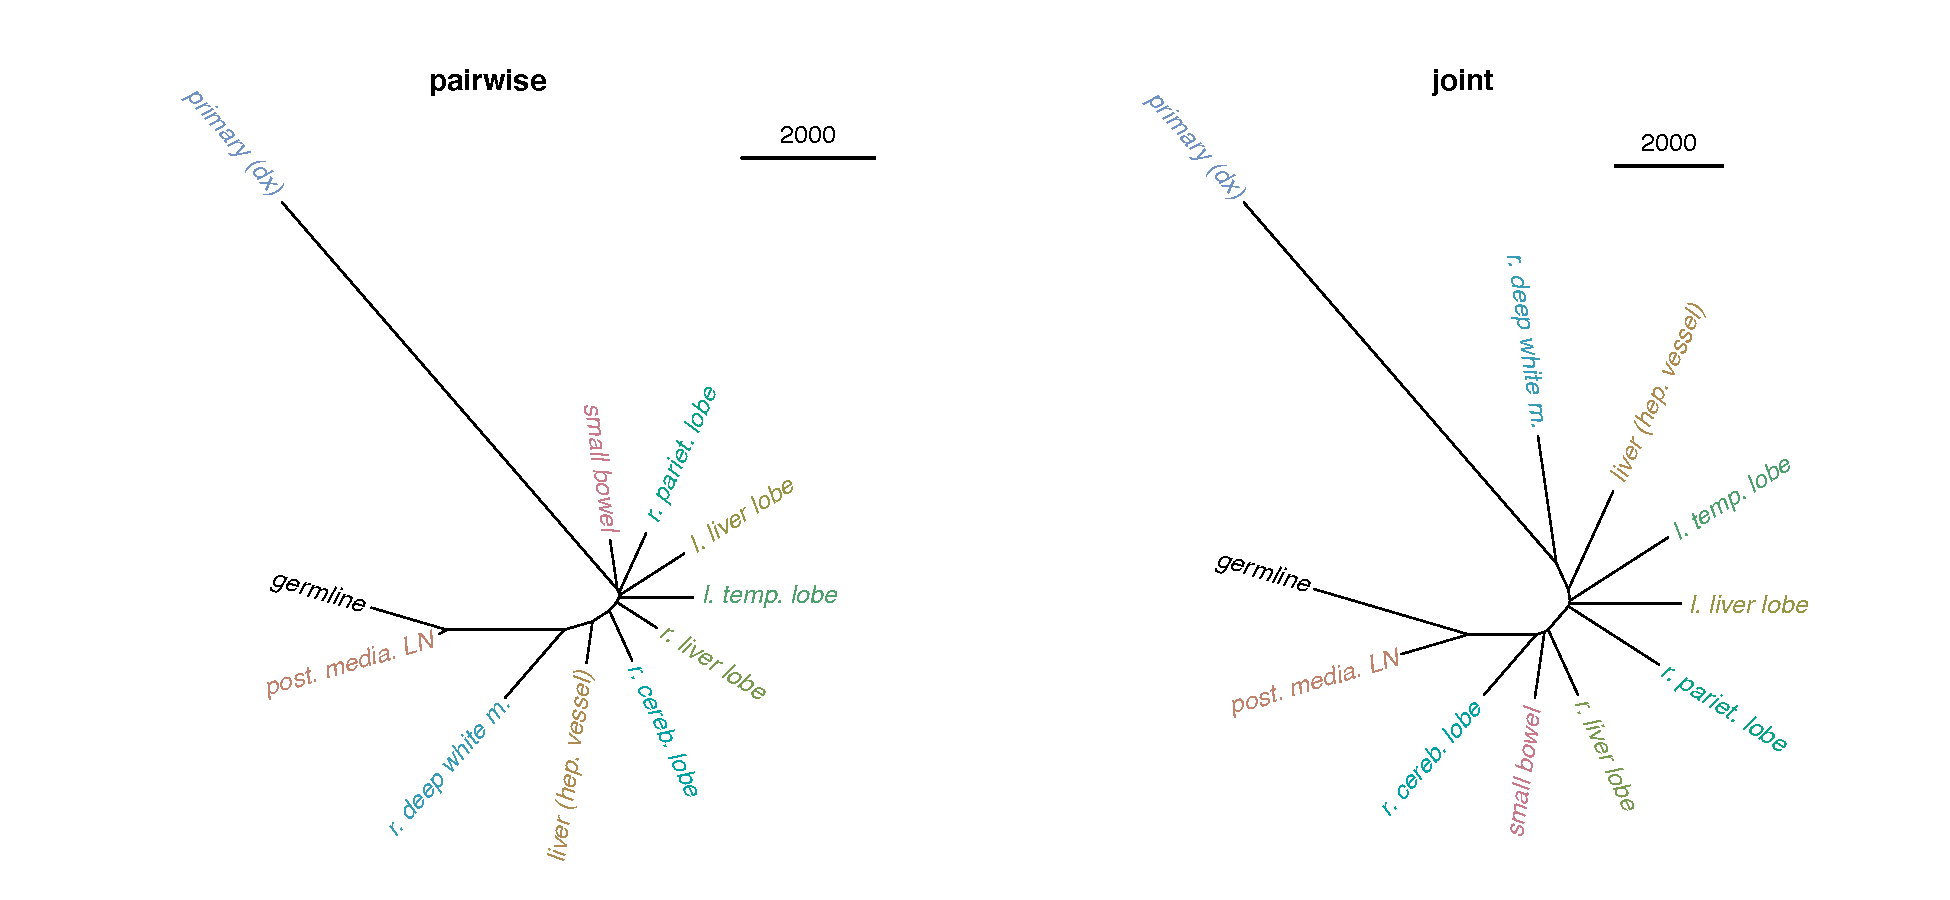
\includegraphics[width=.99\linewidth]{Figures/phyloCA9.pdf}
\caption[Reconstructed phylogenies of joint samples]{Reconstructed phylogenies of a patient with multiple spatially distinct samples; Neighbour joining on Hamming distance on variant occurrence vector. Tip labels describe the location of the sample in the patient. Trees are shown as unrooted with germline as fixated origin point; black line ruler shows the length of an edge with 2000 mutations}\label{fig:ca9phylo}
\end{figure}

\todo[inline, color=green]{Maybe adjust the font size in the trees to make it more readable}

There are several obvious changes, first, the longer edge connecting the the germline, which we consider as the state of no somatic variants, to all other samples. This shows that there are many more shared mutations in all samples, than what would have been anticipated with the default method, which corresponds to an overestimation of the heterogeneity of the samples. As the accumulation of somatic variants is still used as a proxy for timing and cell divisions, when assuming a high mutation rate for lung cancer ($5.3 \cdot 10^{-8}$ from \citeauthor*{Werner2020} \cite{Werner2020}) this difference of $\approx 36000$ variants is equivalent to $\approx 2000$ cell divisions. While the cell doubling rate of lung cancers is highly dependent on the type \cite{Arai1994}, this difference makes a huge difference when assessing the timing of the tumour initiation and further evolution. 

Secondly, there have been topological changes, which generate a longer bifuricating edge between the olive coloured ``r. liver lobe`` and the ``r. pariet. lobe`` showing a bottle neck in cancer evolution, which fits very well with the clinical history, where the patient lived with stable disease for almost ten years, before progressing and dying. The extreme distance of the primary/diagnostic sample from the rest of the samples could be either a difference in sequencing quality, or due to the exposure to FFPE for the ten years between tumour diagnosis and death. However, as this feature is preserved between both the joint and the pairwise analysis it is no result of our new method.

\begin{figure}[!ht]
\centering
\includegraphics[width=.99\linewidth]{Figures/tanglePhyloCA9.pdf}
\caption[Tanglegram of the reconstructed phylogenies]{Side by side view of the reconstructed trees from \autoref{fig:ca9phylo}; internal edges, which are distinct between trees are shown as dotted lines; common subtree is shown in red  Tree labels have been sorted to minimise distance between labels; Visualisation generated with dendextend \cite{Galili2015}}\label{fig:tanglePhyloCA9}
\end{figure}
\todo[inline, color=green]{maybe increase the line width of the edges}

\autoref{fig:tanglePhyloCA9} shows a topology focused view of the two trees, which highlights the breaks which are needed to morph one tree into the other with dotted edges \cite{Vienne2018}. The common subtrees are coloured the same on both sides and connecting lines show identical labels. This format shows that while the trees look quite similar at first glance, they show vastly different topologies.


One example of this is ``small bowel`` which was connected to the red common subtree, but is now much closer to the ``r. cereb. lobe`` and forms a parallel clade with the ``r.liver lobe``. In general, where the pairwise tree shows a very linear topology, which leaves only branching out of the main with no disjunct subclades, which are clearly present in the joint reconstruction.  (\autoref{fig:tanglePhyloCA9}).


\section[Longitudinal analysis]{Longitudinal analysis - something for the ages }
\label{variantcalling-sec:longitudinal}

While the initial motivation for the development of these workflows was the analysis of multi-region, so spatial, samples from the same patient coming from the CASCADE rapid autopsy program, a longitudinal application of these methods for the joint analysis of diagnostic and relapse sample, or even the repeated testing of ctDNA are quite worth thinking about. In this part, I will present work using the published workflows on a longitudinal dataset, which highlights the flexibility and wide spread usability of the new methods.

In addition to their autopsy, Patient ``CA-F`` also had three longitudinal blood samples taken, from which ctDNA was extracted and WES performed. In a study of late stage melanoma patients, \Citeauthor{Tan2019} identified ctDNA sequencing as a way to stratify patients into high and low risk of relapse and therefore inform adjuvant therapy \cite{Tan2019}, which makes this patient a prime example to show the improvement with joint variant calling. Similar to the spatially related samples, the joint analysis can improve the performance, which then in term enables the detection of lower allele frequency variants, either through lower tumour burden or through the limited availability of DNA fragments from brain lesions due to the blood brain barrier \cite{2014}.

To show that even in longitudinal data, the joint analysis can boost the signal, we jointly variant called the diagnostic biopsy with only the three ctDNA samples and compared them with the results from the pairwise analysis. On average we found 2905 additional variants in each of the ctDNA samples which is more than double than the average number of variants found with the pairwise analysis (2414). Out of those, we found 534 variants in the ctDNA samples, which were found as a high confidence variant in the diagnostic sample, indicating that these findings are high quality calls. 

\begin{figure}[!ht]
\centering
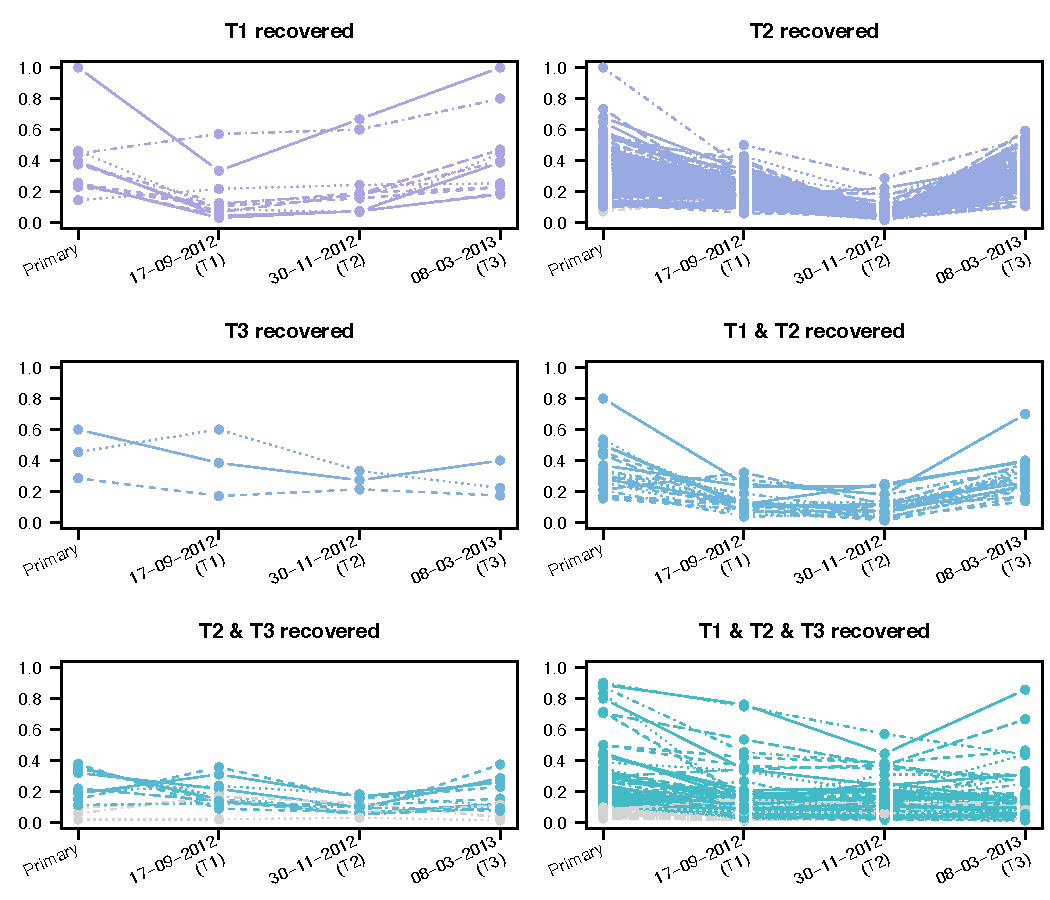
\includegraphics[width=.99\linewidth]{Figures/longitudinalCA9ctDNAVafs.pdf}
\caption[Improved somatic variant calling in longitudinal data]{Improved somatic variant calling in longitudinal data: Variant allele frequency (VAF) of variants found additionally through joint variant calling which were found as high confidence variants in the primary sample; Variants with less than 0.1 VAF in the primary are coloured grey; ``T1 recovered`` shows variants, which were high confidence in all ctDNA samples but T1 and were only found through joint calling there; Axis label show the date of blood collection }\label{fig:longitudinalVAFsctDNA}
\end{figure}

Exactly like in the spatially different samples, in longitudinal data lower tumour purity samples benefit more from the joint analysis. We see that time point 2 (T2) has the highest amount of recovered variants (377) which are found as high confidence variants in both other time points (\autoref{fig:longitudinalVAFsctDNA} A vs. B vs. C) and T2 also has the lowest tumour purity in the cfDNA recorded (T1: 60\%; T2: 20\%; T3: 60\%) however, there are still 106 variants, which were not found in the ctDNA samples at all with the pairwise analysis at all, even though they were high confidence variants in the primary sample (\autoref{fig:longitudinalVAFsctDNA}F). These variants usually show a lower depth of coverage (dp) in the ctDNA samples, which might indicate a problematic region in the genome, but rather than it not being called a variant, it is just a sign of incomplete data, which can be used with our joint approach. 

\begin{figure}[!ht]
\centering
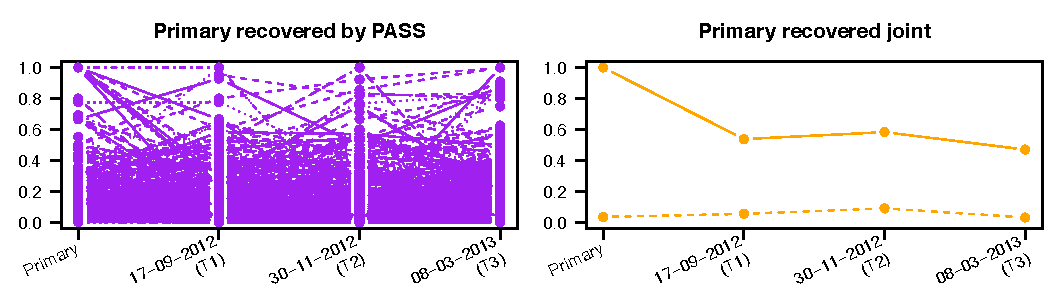
\includegraphics[width=.99\linewidth]{Figures/longitudinalCA9primaryVafs.pdf}
\caption[Longitudinal data informs diagnostic variant calling]{Longitudinal data informs diagnostic variant calling: Vafs of variants additionally found through joint calling in the primary samples; Primary recovered by PASS shows variants which were high confidence in at least one ctDNA sample; Primary recovered joint shows variant which were low confidence in all samples in the pairwise analysis; Axis label show the date of blood collection}\label{fig:longitudinalVAFsprimary}
\end{figure}


Finally, we can also find 398 additional variants in the   primary sample. 398 were discarded due to missing data in the the tissue sequencing, but could be found with a high confidence in the longitudinal data and two of the variants were included, as all 4 samples had this variant below the detection threshold (\autoref{fig:longitudinalVAFsprimary}). The missing depth in the primary also leads to the occasional very high allele frequency of the variant, as all available reads show the variant, but their numbers are below the threshold normal variant callers will report variants.

This shows that both spatially and longitudinal related samples should be analysed jointly, as it substantially increases the amount of true variants found, which as shown before have a big impact on downstream analysis of the samples.



\subsection[Clonal deconvolution]{Clonal deconvolution}
\label{variantcalling-sec:clonal}

Finally, the holy grail of analysis of multiple related samples from the same patient is the clonal deconvolution, where subclonal reoccurring patterns of mutations (clones) are resolved both spatially and longitudinally. These reoccurring clones can be linked to either parallel evolution through positive selection pressure, like a targeted drug, or to the process of developing Metastases where a piece of the cancer ``breaks`` off and grows at a different site.
Surprisingly, as it shares the same issue as the joint somatic variant calling of needing deeply sequenced data from multiple samples of the same organism, there is a plethora of algorithms and methods available for clonal deconvolution. Since 2015 PhyloWGS \cite{Deshwar2015}, Canopy \cite{Jiang2016}, CLOE \cite{Marass2016}, CloneFinder \cite{Miura2018}, MACHINA \cite{ElKebir2018} and MOBSTER \cite{Caravagna2020} were published, to name a few. Underlying all these models is a form of clustering variants with similar variant allele frequency together, to reduce the combinatorial space and enhance the confidence in the signal \cite{Tarabichi2021}. However due to the high number of tools, the challenge to select the right tool is substantial, especially since all of them have up and downsides \cite{Miura2020}. In this work I decided to use PhylogicNDT \cite{Leshchiner2018} as it has been shown to work well on clinical samples \cite{Gerstung2020} and does not have the restriction for the input to be from copy number neutral areas which many of the other tools have.

The analysis was conducted by transforming the variants called with the joint workflows as well as the default pairwise analysis into the required file format without the cancer cell fraction part, in order to let PhylogicNDT calculate those on the fly. The local copy numbers for each variants are generated by intersecting the called segments from sequenza with the position of the variants. Variants which could not be assigned a local copy number change were discarded from the analysis.

\begin{figure}[!ht]
\centering
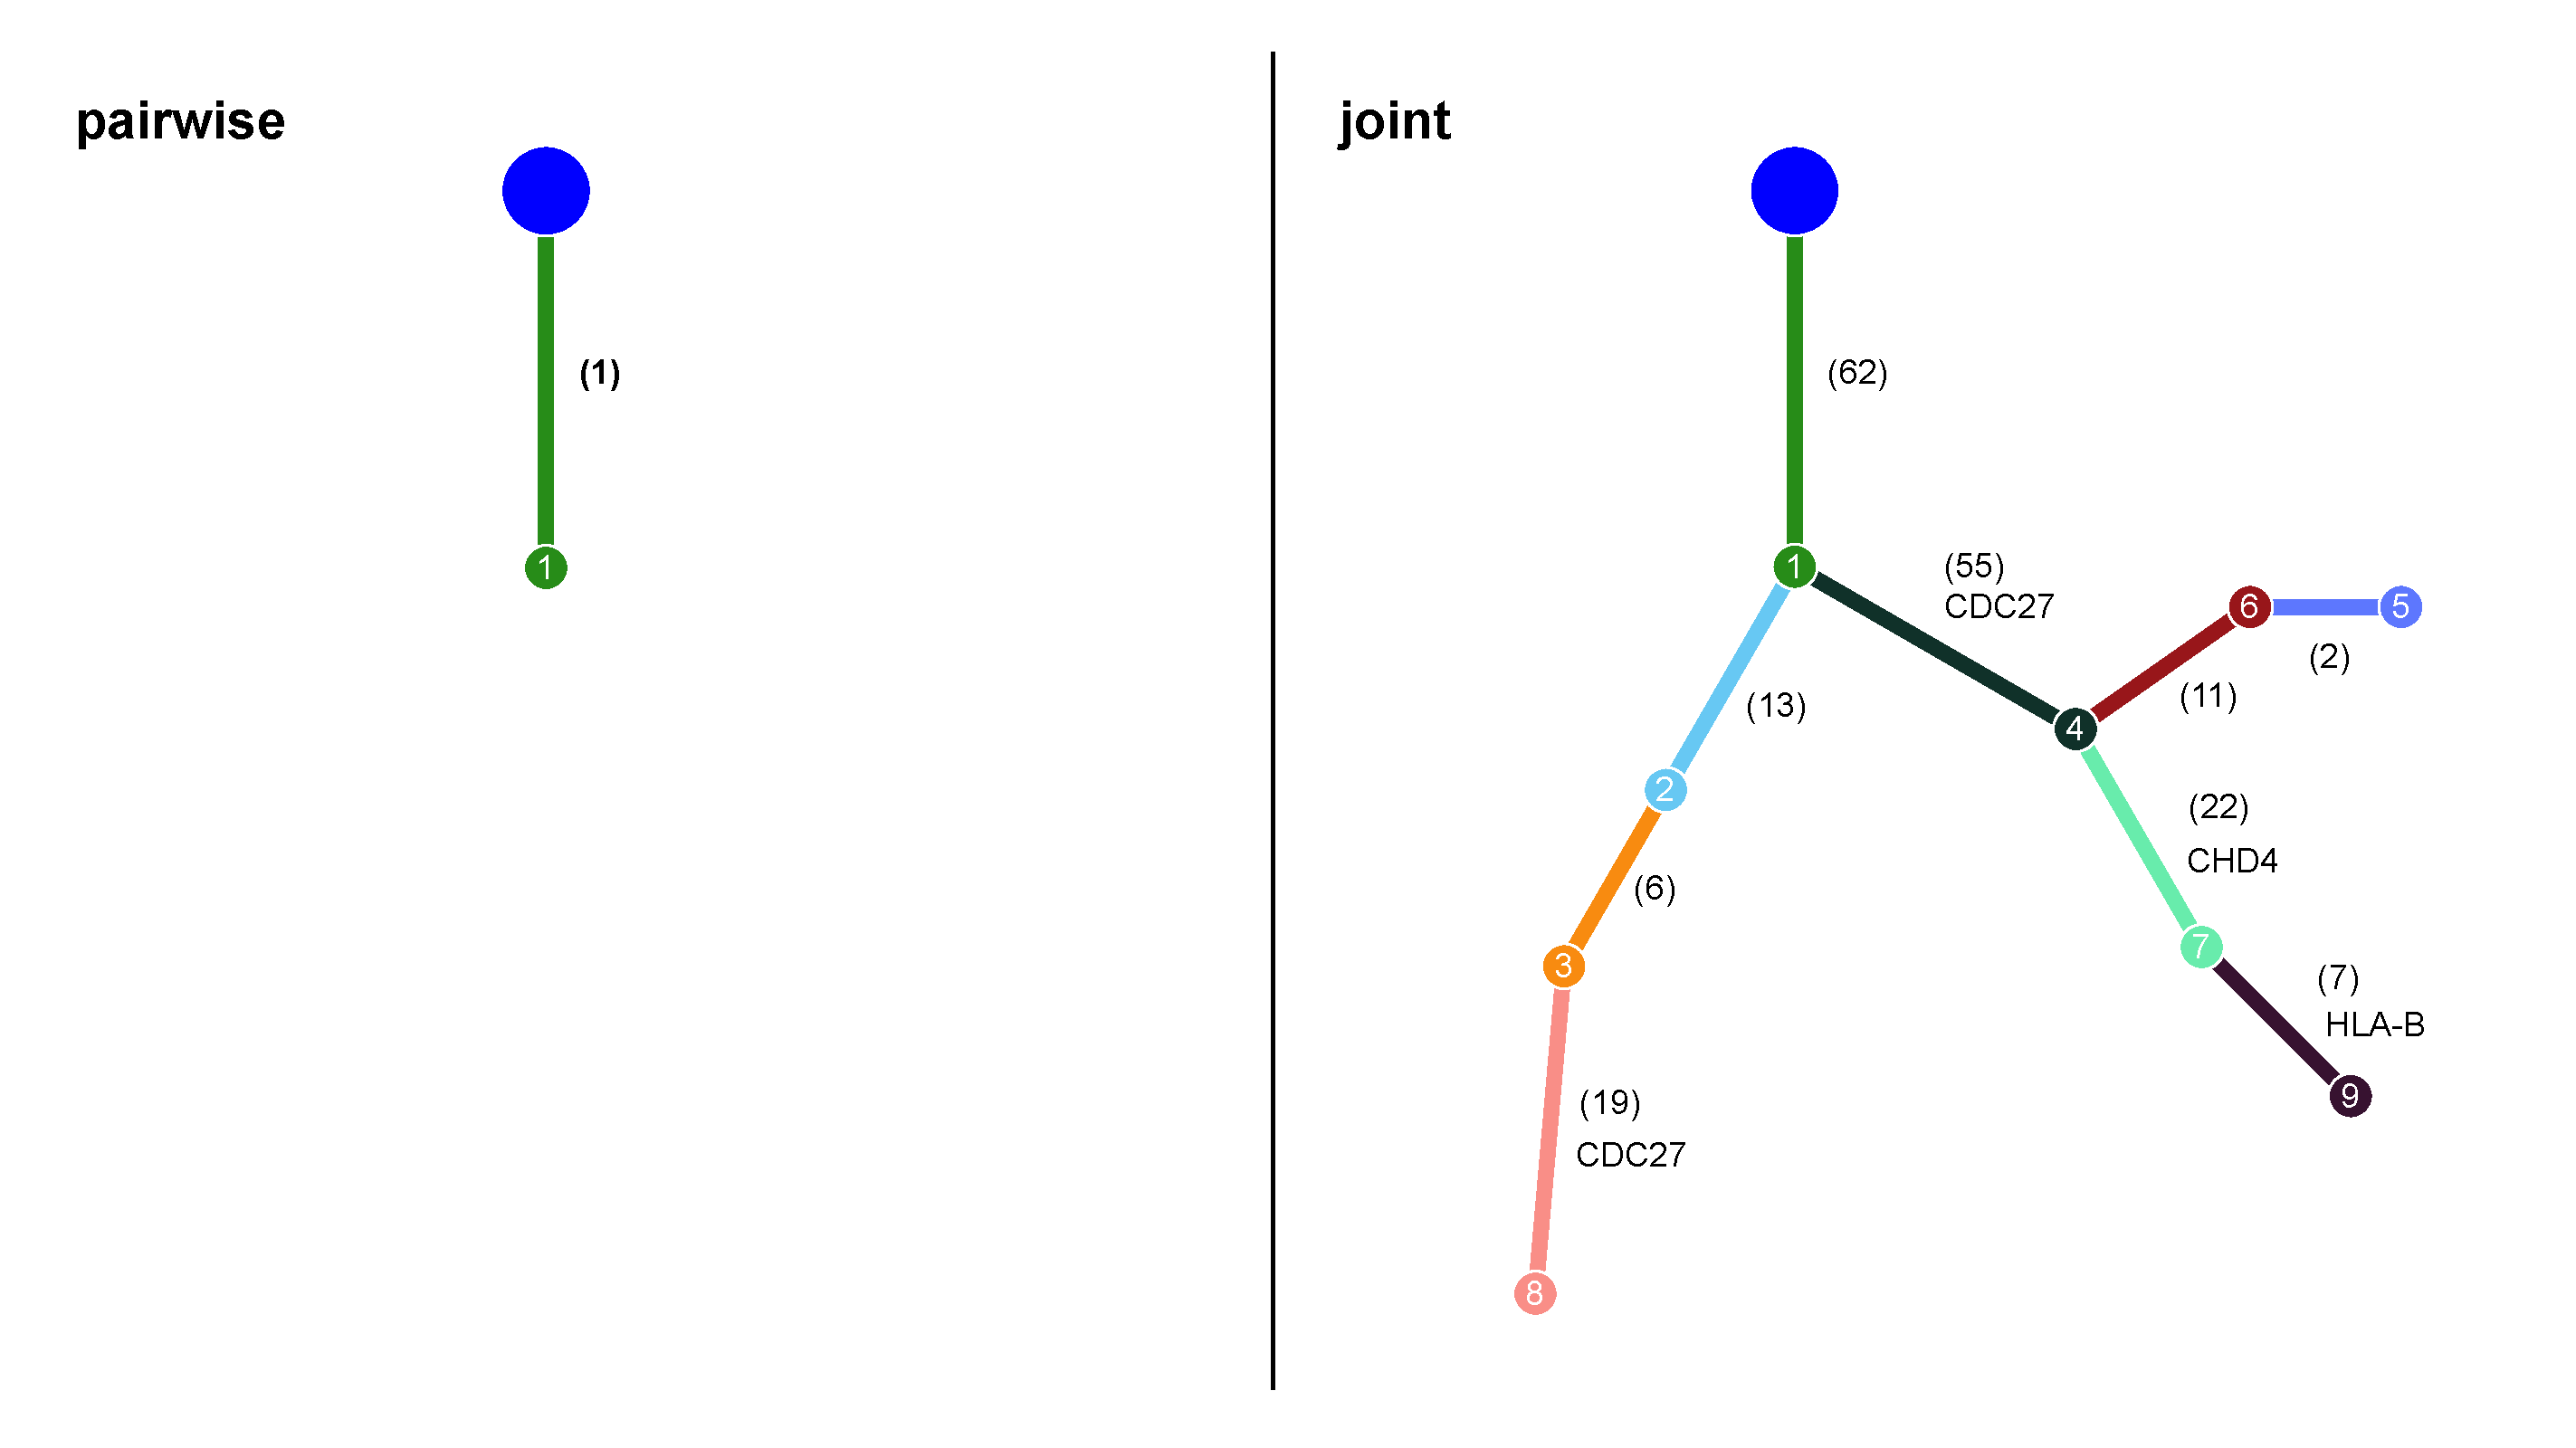
\includegraphics[width=.99\linewidth]{Figures/clonalDeconv.pdf}
\caption[Reconstructed clonal trees for joint and pairwise variant calling]{Reconstructed clonal trees from PhylogicNDT; Blue circle at top depicts the germline/normal state. The coloured edges with the same coloured circle represents a distinct subclone of the parent from which the edge emerges; The number in braces next to the edge is the number of mutations which define this subclone with an added gene symbol added, if there is a cancer driver gene mutation. The left part shows the result when using the default pairwise method of Strelka2 and the right side uses the results from the Strelka2Pass workflow}\label{fig:clonaldeconv}
\end{figure}


\autoref{fig:clonaldeconv} shows the highest parsimony clonal tree reconstructed by PhylogicNDT for the pairwise as well as the joint variant calling. As the copynumber calling information is the same for both inputs, the only difference is in the called variants. While there was no subclonal structure detected at all for the pairwise analysis, there is a highly variable structure detected using the jointly called variants. As this is a clinical sample, we cannot 100\% be sure that the more branched model is the actual truth, but its biologically more logical that a late stage cancer has developed several subclones, rather than it being a very homogeneous disease at all of the 10 sites at autopsy with no evolution over ten years of disease \cite{Gerstung2020}.
It is of particular interest, that the \textit{CDC27} gene got mutated at different time points in different clones (clone 8 vs. clone 4), which a clear sign of parallel evolution, which would definitely be missed without the joint analysis.


\subsection{Longitudinal enriched phylogeny}
\label{variantcalling-sec:fullphylo}
Of course it is finally also possible to build a phylogeny with both the spatial tissue samples as well as the longitudinal ctDNA samples. However, as the ctDNA give a holistic view of all cancer metastases (\autoref{intro-sec:ctDNA}) the interpretation needs to accommodate for that. 

\begin{figure}[!ht]
\centering
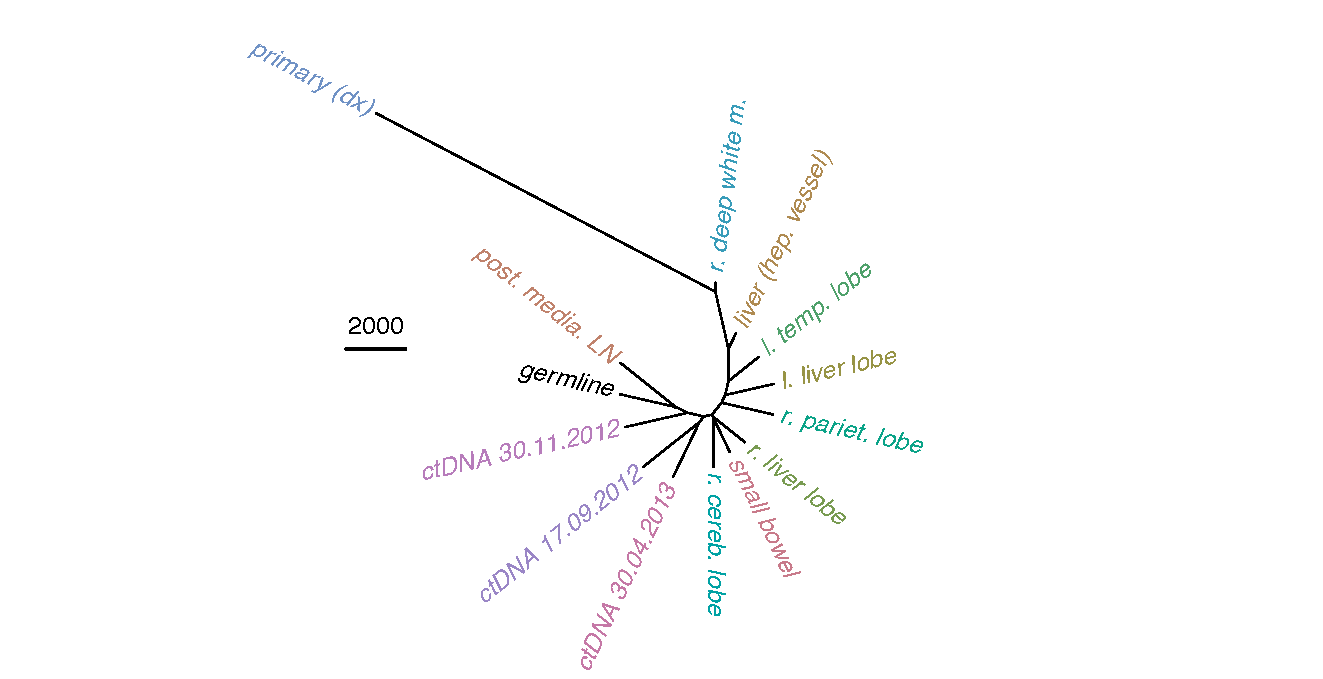
\includegraphics[width=.99\linewidth]{Figures/phyloCA9_withctDNA.pdf}
\caption[Reconstructed phylogeny with longitudinal ctDNA samples]{Reconstructed phylogeny with longitudinal ctDNA samples: Tree from \autoref{fig:ca9phylo} with three additional ctDNA samples from different time points about one year prior to death. Ruler shows the equivalent of 2000 mutations} \label{fig:phyloCA9ctDNA}
\end{figure}

The maybe most surprising thing is that the more temporally distant ctDNA samples from 17.09.2012 and 30.04.2013 are in a subclade together, away from the ``ctDNA 30.11.2012`` sample. Secondly, the addition of the ctDNA samples also lead to a further bipartition edge, which separates ``r. liver lobe``, ``small bowel`` and ``r. cereb. lobe`` from the rest of the tree (\autoref{fig:phyloCA9ctDNA}). This was already inferable from the topology of the previous tree in \autoref{fig:tanglePhyloCA9} ``joint``, but is even more pronounced with the inclusion of the ctDNA samples.

This shows again, that the addition of more samples helps to refine and improve the trajectory and history of cancer samples and it is vital to do this analysis jointly to generate the optimal result.

% the info about longitudinal analysis
\section[Longitudinal analysis]{Longitudinal analysis - something for the ages }
\label{variantcalling-sec:longitudinal}

\todo[inline]{Consider the order of longitudinal vs downstream}

While the initial motivation for the development of these tools was the analysis of multi-region, so spatial, samples from the same patient coming from the CASCADE rapid autopsy program, a longitudinal application of these methods for the joint analysis of diagnostic and relapse sample, or even the repeated testing of ctDNA are quite worth thinking about. In this part, I will present work using the published workflows on other datasets, which highlights the flexibility and wide spread use of our new methods.

\todo[inline]{select the right dataset to show here (possibly the one from the MisMatchFinder stuff)}

% usage of the tool
\section[Usage]{Usage - its not just me that thinks it is good}  

% contains all the links for the cascade chapter
\chapter[CASCADE]{CASCADE - Late stage lung cancer in the spotlight}
\label{ch:cascade}

% intro for the chapter
\section{Introduction}
\label{cascade-sec:intro}

\todo[inline]{talk about cascade autopsies}

\subsection{Lungcancer}
\label{intro-sec:lungcancer}

With around 1.6 million deaths world-wide each year, lung cancer is the number one cause of cancer death \cite{Siegel2018}. Every year about twelve thousand Australians get diagnosed with lung cancer. These cases can be generally split into two groups: small cell lung cancers (SCLC) and non-small cell lung cancers (NSCLC), which account for around 15\% and 85\% of cases, respectively. The majority of NSCLC are either lung adenocarcinoma or lung squamous cell carcinoma \cite{Molina2008}. Even though smoking is highly associated with lung cancers, there is a big group of never smokers, with a high risk of lung cancers in East Asia, especially women, which is correlated with outside influences like pollution and occupational carcinogens and paired with genetic susceptibility \cite{Sun2007}.
This group usually shows \textit{EGFR} (epidermal growth factor receptor) driven tumours. EGFR is a transmembrane receptor tyrosine kinase, which is usually only expressed in epithelial, mesenchymal, and neurogenic tissue, but its overexpression in other tissues is a hallmark of many human malignancies, not just NSCLC.


%% original abstract
%Approximately 50% of patients with non-small cell lung cancer (NSCLC) develop acquired resistance to EGFR tyrosine kinase inhibitors (TKIs) through mutations in EGFR T790M. Maintaining a dynamic balance between T790M positive and negative clones offers an opportunity to delay the emergence of resistance and improve disease outcomes. It is now possible to quantify EGFR mutations using circulating tumour DNA (ctDNA) which can provide a surrogate measure of clonal populations within tumours. This project will utilise next generation sequencing (NGS) of tumour tissue and ctDNA in patients treated with EGFR TKIs to study clonal evolution patterns and predict optimal treatment approaches to delay therapeutic resistance.

% the publication (maybe also Marian's publication)
\section{Publication}
\label{cascade-sec:publication}

% the analysis done as a total cohort


\section{Cohort level analysis}
\label{cascade-sec:cohortLevel}

Even though there were only five lung cancer patients who have participated in the CASCADE program to date, each of the patients had a high number of samples analysed, revealing the complexity of intra-patient heterogeneity in NSCLC (\autoref{cascade-sec:patientLevel}). Despite this heterogeneity, there were several parallels between the patients showing similarities in disease trajectories. The process of small cell transformation (SCT) is still significantly under explored and understood, due to the rarity of the transformation as well as the lower overall survival in comparison to other resistance mechanisms. In the following section, the patients who developed small cell carcinoma transformation were compared and contrasted with the adenocarcinoma cases to further explore this mechanism of resistance.

The generally accepted hallmarks of SCT, apart from the histological changes such as high \textit{MKI67} expression and down regulation of major histocompatibility complex I and II, are a much higher mortality, a high prevalence of \textit{FHIT} and \textit{MAD1L1} deletions or loss, and \textit{TP53} and \textit{RB1} mutations \cite{Meerbeeck2011,Raso2021}. However, while in patient CA-L all samples showed a TP53~``stop gained`` mutation, patient CA-I's transformation did not occur in the setting of  \textit{TP53} loss. Additionally, neither of the patients presented with a \textit{RB1}, \textit{FHIT}, or \textit{MAD1L1} loss (\Autoref{fig:ca51heatmap,fig:ca86heatmap}). 

In agreement with recent literature showing whole genome doubling (WGD) for SCLC \cite{Zhou2021}, we observed chromosomal arm amplification in patient CA-I and full WGD for patient CA-L. However, all NSCLCs patient also showed at least one sample with complete WGD, casting doubt on WGD being a distinguishing feature of SCT (\Autoref{tab:ca99cnv,tab:ca51cnv,tab:ca80cnv,tab:ca82cnv,tab:ca86cnv}). Additionally, the overall loss of heterozygosity could be seen in both NSCLC and SCLC and this seems to be a general feature of late stage lung cancers rather than NSCLC (\autoref{fig:cascadeLOH}) suggesting that copy number alterations are not the main drivers of SCT.

\begin{figure}[ht]
\centering
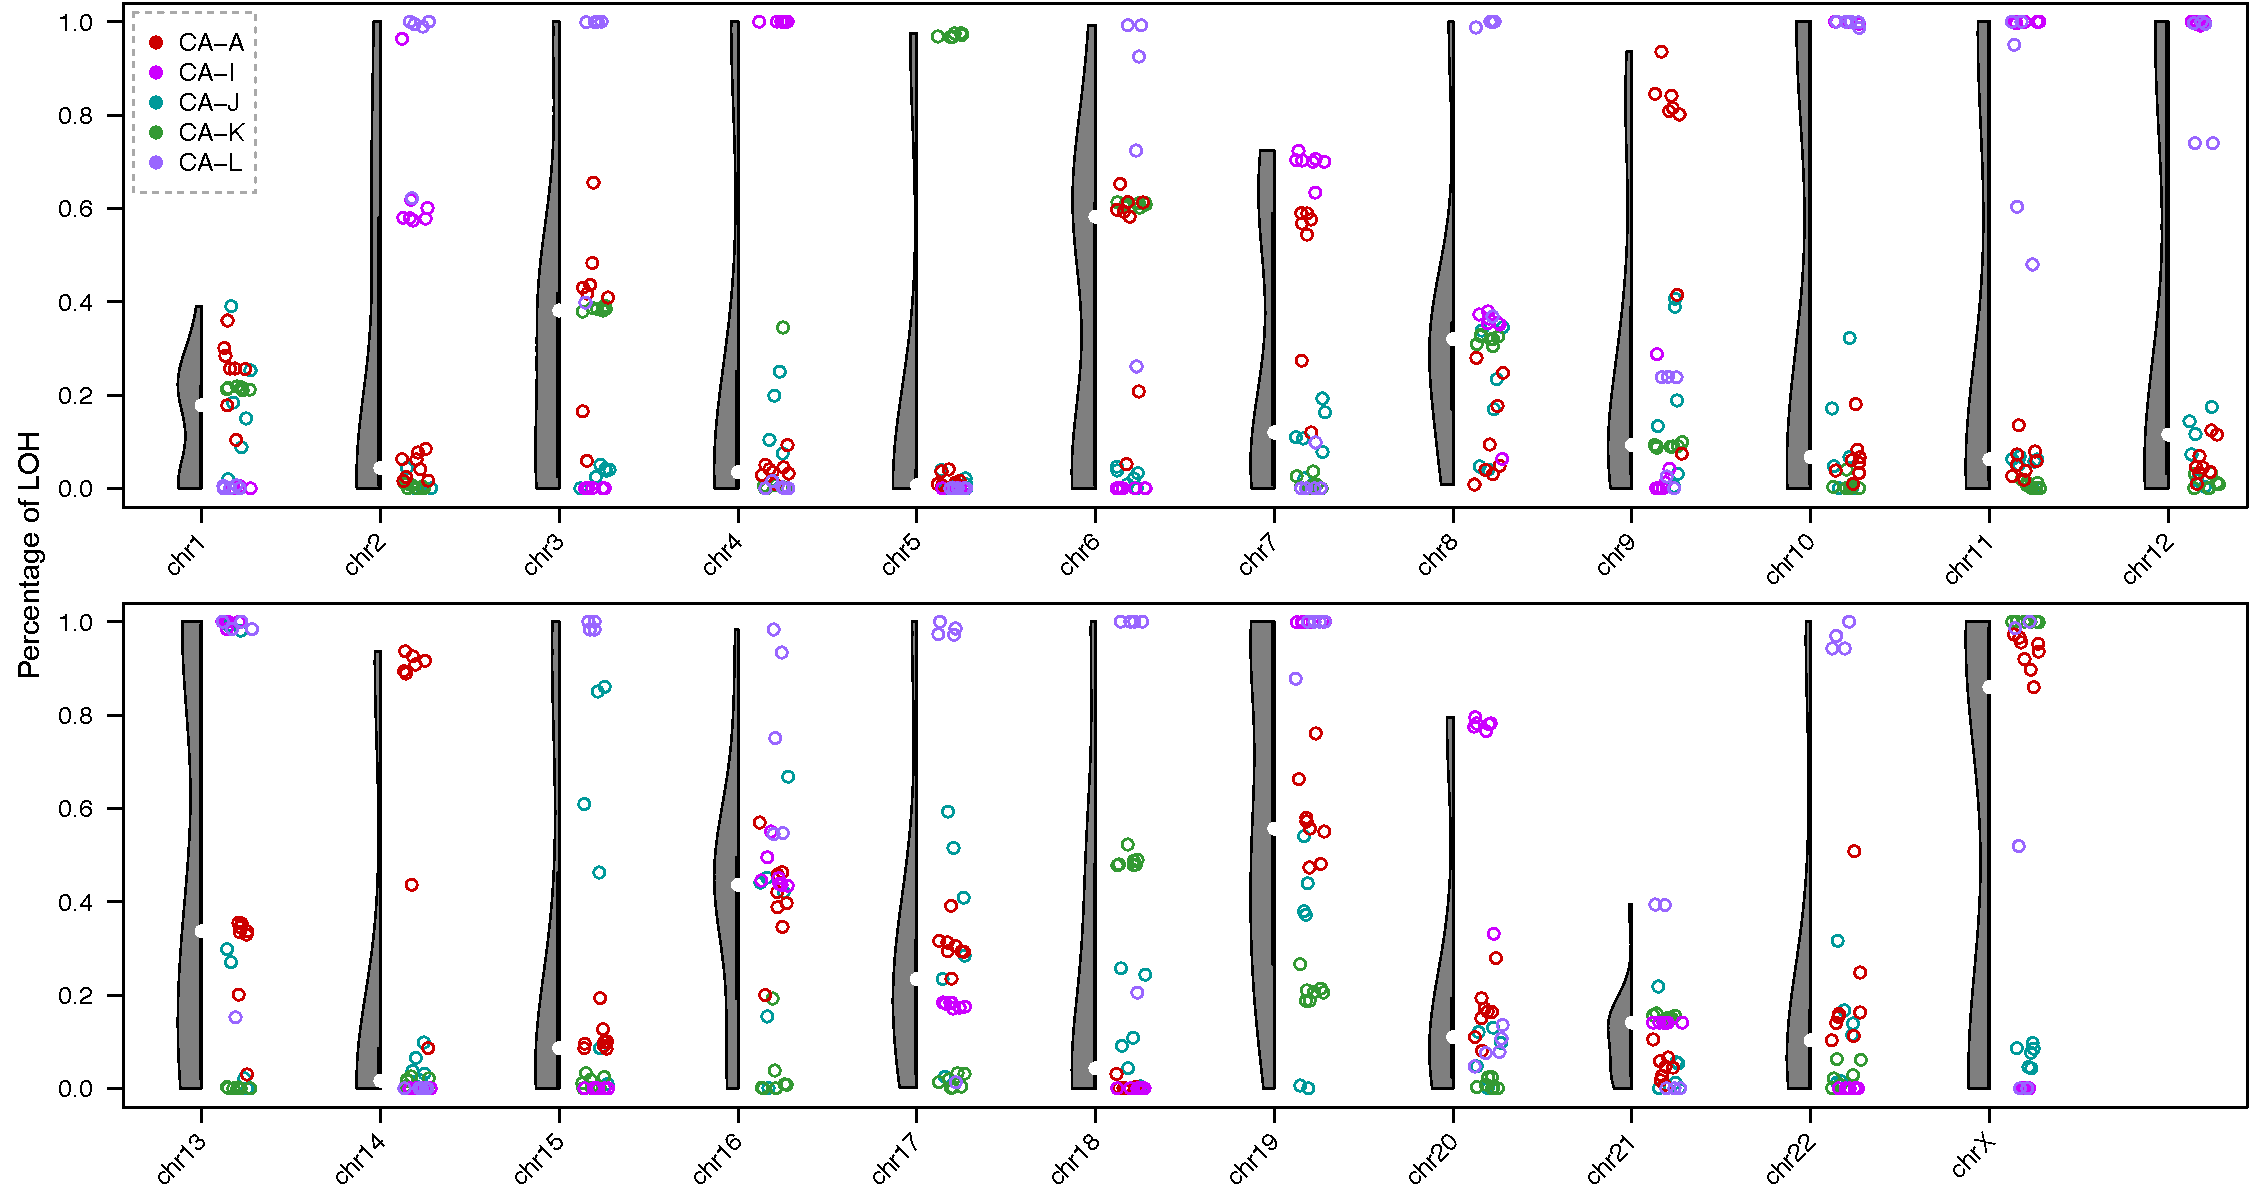
\includegraphics[width=.99\linewidth]{Figures/CASCADE/LOH_perChrom.pdf}
\caption[Percentage of LOH per chromosome in CASCADE patients]{Percentage of LOH per chromosome in CASCADE patients: Per chromosome violin plots are shown in grey with median as white dot; individual percentages per sample are displayed grouped with colour per patient; LOH was called with a major copy number <0.6 and a major copy number > 0.6} \label{fig:cascadeLOH}
\end{figure}


The most prominent difference of NSCLC and SCLC in our patients was the reconstructed phylogeny. While the NSCLC showed substructure and meaningful evolutionary splits, the SCLC patients phylogenies showed a distinct ``star shaped`` pattern. Each sample branch was very close to the others and with substantial amounts of private variants in each sample (\Autoref{fig:CA51mitoPhylo,fig:CA86mitoPhylo} vs. \Autoref{fig:CA99mitoPhylo,fig:CA80mitoPhylo,fig:CA82mitoPhylo}). Even though the shared variants in CA-L seemed to provide the ability to transform, they do not necessitate the transformation, as both samples CA-L 17A and 26 remained NSCLC with virtually no known genetic determinant of status. This in term suggested either a currently undetected genetic determinant or potential epigenetic regulation to explain the SCT (\autoref{fig:ca86heatmap}).

In contrast to CA-L, who presented with both NSCLC and SCLC, CA-I's samples were completely transformed. The biopsied adenocarcinoma, which already had an MHC-I disrupting mutation was completely out-competed by a secondary clone, which did not present with any additional genetic driver alterations. Similar to patient CA-L this suggested, that the genetic prerequisites for SCT were already present in the clonal population, but not sufficient to drive transformation (\Autoref{fig:ca51.clonalTree,fig:ca51.ccfCluster}). 

Gene fusions or regulatory genetic variants leading to aberrant transcription could have been the cause for this phenomenon observed in both SCT cases. These could be detected in RNA sequencing of the biobanked fresh autopsy samples to exclude genetic causes which were not picked up with the performed WES, or detect transcription alterations. However, this analysis is outside the scope of this work.



% the analysis about mitochondrial phyolgenies
\section[Mitochondrial phylogenetic reconstruction]{Mitochondrial phylogenetic reconstruction - the power house of the phylogenies}
\label{cascade-sec:mitochondria}

While phylogenetic reconstruction is a well established method for genetic variants from canonical chromosomes to study metastatic progression and timing of evolutionary divergence \cite{Deshwar2015,Brown2017,Hu2019}, there are multiple issues. In \autoref{variantcalling-sec:phylo} and \autoref{variantcalling-sec:clonal} I showed how important the proper variant calling method is to accurately recover phylogenies and clonal patterns. 

However using somatic variants to reconstruct phylogenies is flawed to begin with, as most models studying genetic variation assume neutral evolution of the sites \cite{Kimura1968,Lynch1989}, but cancers almost exclusively exhibit positive selection \cite{Cannataro2018}. And while passenger mutations might not directly affect fitness of the cell, they only exist due to the link to the driver mutation and therefore has little to no additional information gain in addition to the driver. In addition, while in small populations genetic drift as a stochastic process overpowers selective processes (fitness coefficient $s$) and can therefore be assumed to be neutral, in larger populations $N_e$ (effective population size) where \autoref{mmf-eq:neutralSelection} does not hold true, mutations are under selective pressure \cite{EyreWalker2007}.
\begin{equation}
N_e \cdot s \ll 1 \label{mmf-eq:neutralSelection}
\end{equation}
\myequation[\ref{mmf-eq:neutralSelection}]{Selective pressure with effective population size}
%we need to squish this a bit otherwise it looks weird
\vspace{-3em}
All in all we can assume that with cancer growing, positive selection through treatment and tumour micro environmental niches, almost all assumptions of the coalescent theory are not applicable for tumour samples and therefore methods using somatic variants and their respective results need to be selected and evaluated carefully.

To tackle this issue, and assist with the interpretation of phylogenetic reconstruction results, we adjusted a method used in single cell sequencing to track clonal expansion with mitochondrial somatic mutations \cite{Ludwig2019} to be usable for standard bulk sequencing. Mitochondrial variants are an ideal source of clonality information, because the mutation rate is significantly higher than nuclear DNA, due to the missing proof reading and repair mechanisms, which allows very granular separation in a shorter time period. Additionally, while there are several diseases cause by defects in mitochondria such as Kearns-Sayre syndrom \cite{Harvey1992}, MERRF \cite{Adam1993} and MELAS \cite{Hirano1992}, they usually follow a mendelian inheritance pattern and are hereditary and not somatically acquired. In the cancer text, somatic mutations in mitochondrial DNA are assumed to be approximately neutral with a possible selection pressure towards healthy ageing and negatively selecting cancer \cite{Rodell2013,Yuan2020}.

\subsection{Method}
\label{cascade-sec:mitoMethod}

First a pileup of all mitochondrial positions is performed. Before the pileup we preselect reads which uniquely map to the mitochondrial genome and only retain high mapping quality reads. Then the nucleotide counts in each position is transformed into a MultiEssayExperiment \cite{Ramos2017} for final analysis in R. The preprocessing code and be found in \autoref{lst-cascadeAppendix:mitoPreProcessing}.

The final MultiEssayExperiment is then read into R and quality metrics applied to exclude samples with not enough coverage on the mitochondrial contig. usually WGS samples will show an extensive coverage of mitochondrial DNA, however WES will require a library preparation with probes in this area. Patient CA-I has a coverage of more than 100x for all but the germline sample which only has an overall coverage of 17x. Similar, patient CA-K \todo{add the stats}. All other Patients (CA-A/J/L) where samples are sequenced as WGS show a coverage of more than \todo{more stats}

\begin{figure}[!ht]
\centering
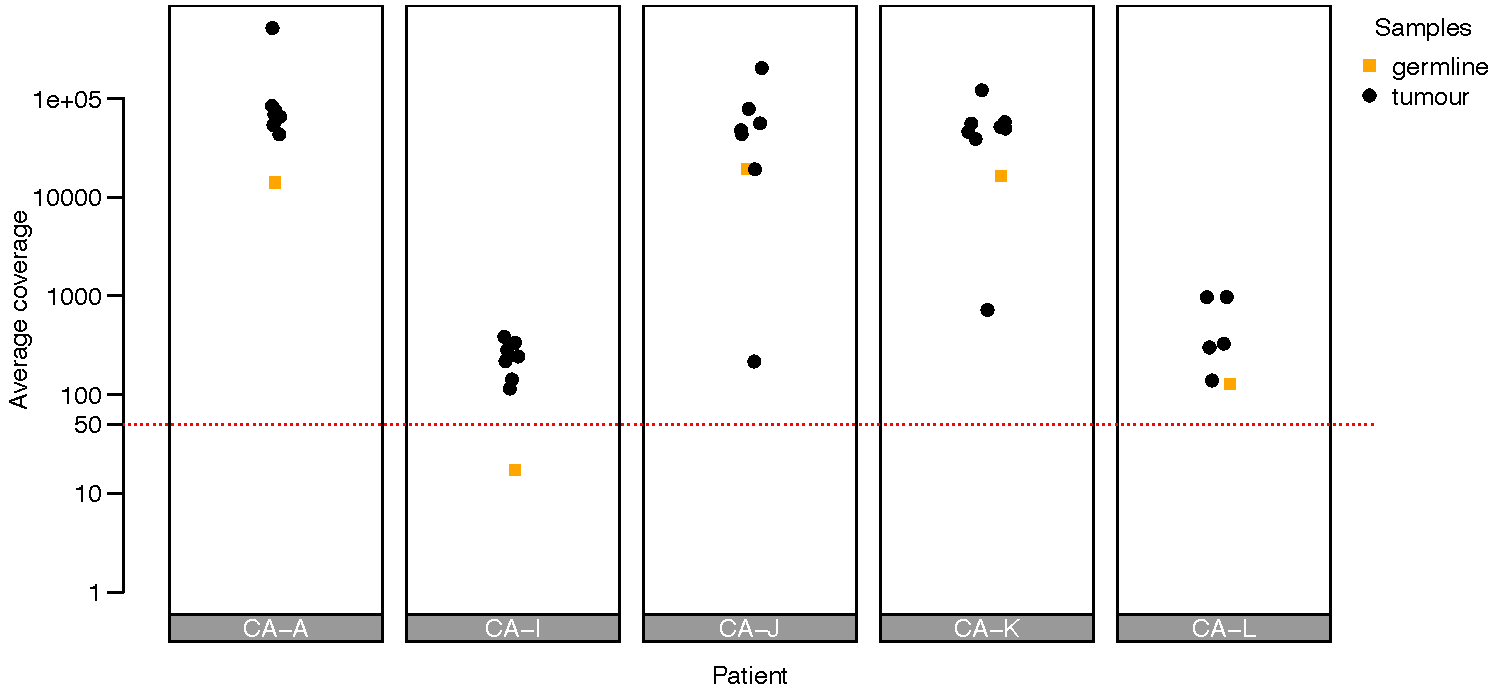
\includegraphics[width=.99\linewidth]{Figures/mtCoverage}
\vspace{-1em}
\caption[Average coverage of mitochondrial DNA of CASCADE patients]{Average coverage of mitochondrial DNA of CASCADE patients: Orange squares show germline sample for each patient; black points show tumour samples; horizontal red dotted line shows quality cut off suggested by \protect\textcite{Ludwig2019}} \label{fig:cas86schematic}
\end{figure}

To ensure optimal results, we will exclude all samples with an average coverage of less than 50x if it is a tumour sample and 15x for a germline sample. If only the tumour internal relations are of interest, the germline sample can also be removed from the analysis in case of lower coverage.


% the missing analysis?
\section{Outlook}
\label{cascade-sec:outlook}

In this chapter we described both the high inter and intra patient heterogeneity of late stage lung cancer patients and showed that mitochondrial phylogeny could help to resolve the sample relationships in the context of selection pressure through treatment. Additionally we uncovered a different disease trajectory of SCLC where the cancer is genetically already transformed, but has not changed histological. This suggested that the early detection of SCT requires the study of pre-transformed SCLC like patient CA-L, to not detect symptoms of the disease and rather the first signs of a potential transformation.

With this work we took a first step towards understanding and measuring the heterogeneity of tumour samples, but many unanswered questions remain. The epigenetic marks and their inheritance patterns in cancer are a massive unexplored field which increases the heterogeneity of cancer even more \cite{Easwaran2014}. Additionally, we could only hypothesis and reconstruct the longitudinal trajectory of the disease from autopsy samples. The next step to validate these findings and explore the hypothesis is to analyse temporally spaced samples from the same disease. 


\begin{savequote}[65mm]
``When the sum is already greater than the parts, there is room to make it greater still.``
\qauthor{--- Navali, Hatungo of the Karui}
\end{savequote}


\chapter[Mismatchfinder]{MisMatchFinder - hope springs eternal}
\label{ch:mmf}

%\epigraph{``Many a mickle makes a muckle.``}{--- \textup{proverb}}

% introduction into the idea of the chapter
\section{Introduction}
\label{variantcalling-sec:intro}

When I started exploring the somatic variant calling methods in the beginning of my PhD in 2018, I was surprised about the stark difference between germline and somatic variant calling methods. Where all "modern" germline variant callers have the built-in capability to joint call multiple samples, for example from family trios, virtually no somatic variant caller had this function.

%description of the methods
\section{Methods}
\label{mmf-sec:methods}

With the change from a variant focused approach to a read based method, this new method will call ``mismatches`` of a read from the reference genome, rather than a variant. This has the advantage of not requiring a matched normal and its use for virtually any sequencing data source, be it TAS, WES, WGS or even nanopore sequencing\footnote{however nanopore is not really usefull due to the short fragments naturally occuring in cfDNA}. However it also means, that the error supression method, which are usually used by variant calling methods like read position ranks sum (RPRS) or strand bias are not useable, which leads to a higher degree of background noise. In the following sections I will describe how we filter and curate the found mismatches to retain as much signal as possible.

\subsection{Data preprocessing}
As this new method has sophisticated internal measures to filter and process sequencing data, the steps for preprocessing are minimal: The reads only need to be aligned to a reference genome (\autoref{intro-sec:mapping}). For optimal mapping and additional noise reduction, paired end sequencing of at least 75 bp is suggested. This ensures a few bases overlap on the standard fragment length of less than 150b of ctDNA (\autoref{intro-sec:ctDNA}). Another optional suggested step is the duplication marking of the BAM file.

\subsection{Mismatch detection}
In contrast to conventional variant calling approaches, which find regions of interest through pileups (position wise) and then realign reads in the surrounding area, to accurately estimate the most likely event that lead to the observed haplotype (\autoref{intro-sec:variantcalling}), with this new method, we take every individual read as a separate entity to fully span the heterogeneity of all cells and their genetic background. A sequencing reads ``MD``- and ``CIGAR``- tag from the preprocessed BAM file are used to reconstruct the sequence of the read and the positions, where the read shows a different base than the reference. These potential mismatch sites will then filtered in multiple steps to reduce the impact of both germline variants as well as sequencing errors

\subsection{Filtering steps}
Apart from the filters, which most variant callers will employ, like mapping quality (MQ) and base quality (BQ), which are used to ignore reads as well as positions respectively, the method also internally filters out common sequencing errors next to homopolymer regions \cite{Heydari2019}. While these cutoffs were preselected by me for optimal performance on our data (MQ=20, BQ=55, homopolyLength=5), the program allows the user to adjust them to their liking.
This is also possible for both the region of interest (ROI) bed-file which was used to restrict the analysis to only highly mappable regions of the genome (\autoref{ch-mmfAppendix:bedfiles}), as well as for multiple other parameters which are unique to our method, like minimum average base quality, minimum and maximum number of mismatches per read and/or fragment, and the minimum and maximum length of a fragment. If any of these values are not within the specified range a read will be discarded in the analysis. This is also the default for reads which have a secondary alignment position or are considered duplicates of any kind.

\subsection[Consensus reads]{Consensus reads - what happens when the sequencer isn't sure}
\label{mmf-sec:consensus}

\todo[inline]{write about the consensus building process with some figures}

% more things, when the story is clear if i just write what i have done and no publication 

\chapter{Conclusion}
\label{ch:conclusion}

\epigraph{``As you think, so you become…..Our busy minds are forever jumping to conclusions, manufacturing and interpreting signs that aren’t there.``}{--- \textup{Epictetus}, The Enchiridion} % 

%% ----------------------------------------------------------------
% Now begin the Appendices, including them as separate files

\addtocontents{toc}{\vspace{2em}} % Add a gap in the Contents, for aesthetics

\appendix % Cue to tell LaTeX that the following 'chapters' are Appendices

%\input{Appendices/AppendixA}	% Appendix Title

%\input{Appendices/AppendixB} % Appendix Title

%\input{Appendices/AppendixC} % Appendix Title

\addtocontents{toc}{\vspace{2em}}  % Add a gap in the Contents, for aesthetics
\backmatter

%% ----------------------------------------------------------------
\label{Bibliography}
\fancyhead[LE,RO]{Bibliography}  % Change the left side page header to "Bibliography"

\printbibliography

\end{document}  % The End
%% ----------------------------------------------------------------
